\sect{5. Cómo se juega}

Tú y tu compañero conducís el coche de persecución de \textbf{Chase H.Q.}, la unidad especial de investigación. En cada una de las cinco fases un criminal huye en su coche. Al empezar la fase, Nancy te dice por radio quién es. Después:

\begin{enumerate}
\item \textbf{Alcánzalo.} El contador \texttt{DISTANCE} muestra a qué distancia va, y tienes \textbf{60 segundos}. Adelanta al tráfico y no te salgas de la carretera.
\item Cuando aparece a la vista sale \texttt{SIGHTING OF TARGET VEHICLE}, empieza a sonar la \textbf{sirena} y el reloj vuelve a \textbf{60 segundos}.
\item \textbf{Embiste su coche} una y otra vez. Cada golpe vacía un poco el medidor de daños que hay a la izquierda de la carretera; después de \textbf{20 golpes} se rinde, se para en el arcén y queda detenido.
\end{enumerate}

\begin{figure}[H]
\centering
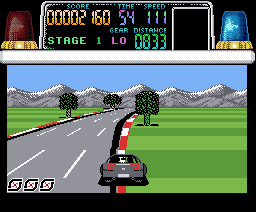
\includegraphics[width=0.48\textwidth]{../img/stage1.png}\hfill
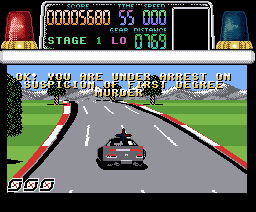
\includegraphics[width=0.48\textwidth]{../img/arrest.png}
\caption{Izquierda: la persecución en la primera fase. Derecha: la detención.}
\end{figure}

\textbf{En la carretera.} Si chocas con otro coche o con algo del borde (árboles, señales, vallas), das un trompo y pierdes velocidad. Fuera de la carretera el coche traquetea y frena. La carretera pasa por túneles y a veces se divide en dos. Si vas demasiado despacio mucho rato, tu compañero protesta.

\textbf{La radio.} La línea bajo el marcador muestra lo que se dice por radio, letra a letra, con la cara de quien habla: Nancy, tu compañero o el criminal.

\textbf{Tiempo agotado y continuar.} Si el reloj llega a cero sale \texttt{TIME UP}. Si te quedan créditos, \texttt{CONTINUE THIS MISSION} cuenta desde 10: pulsa \textbf{MARCHA} antes de que llegue a 0 para seguir con 60 segundos y tres turbos, pero el coche del criminal queda reparado. Tienes \textbf{dos créditos} por partida. Sin créditos, o si dejas que la cuenta termine, se acaba la partida.

\begin{figure}[H]
\centering
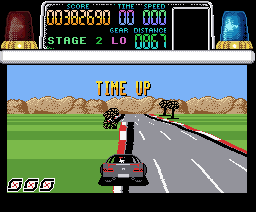
\includegraphics[width=0.48\textwidth]{../img/timeup.png}\hfill
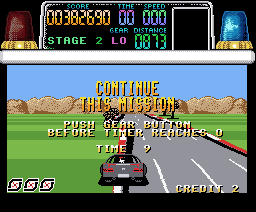
\includegraphics[width=0.48\textwidth]{../img/continue.png}
\caption{Izquierda: se ha agotado el tiempo. Derecha: la ocasión de continuar.}
\end{figure}

% ==================================================================
\sect{6. El marcador}

\begin{figure}[H]
\centering
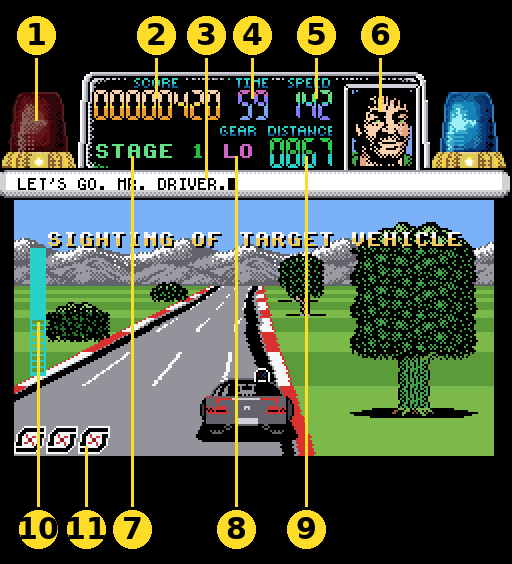
\includegraphics[width=0.9\textwidth]{img/hud.png}
\caption{El marcador de la parte de arriba y lo que se ve en la carretera.}
\end{figure}

\begin{tabularx}{\textwidth}{@{}cp{3.1cm}X@{}}
\toprule
\textbf{\tNo} & \textbf{\tElement} & \textbf{\tTellsYou}\\
\midrule
1 & Sirenas & Las dos luces de policía. Destellan mientras suena la sirena, desde que el criminal está a la vista.\\
2 & \texttt{SCORE} & Tus puntos.\\
3 & Radio & Lo que se dice por radio, letra a letra.\\
4 & \texttt{TIME} & Los segundos que quedan.\\
5 & \texttt{SPEED} & Tu velocidad en km/h.\\
6 & Cara & Quién habla por radio: Nancy, tu compañero o el criminal. Interferencias mientras se sintoniza.\\
7 & \texttt{STAGE} & La fase que juegas, de 1 a 5.\\
8 & \texttt{GEAR} & La marcha puesta: \texttt{LO} o \texttt{HI}.\\
9 & \texttt{DISTANCE} & A qué distancia está el criminal.\\
10 & Medidor de daños & Aparece cuando el criminal está a la vista: cuánto aguanta todavía su coche. Baja con cada golpe; cuando se vacía, queda atrapado.\\
11 & Turbos & Los turbos que te quedan en esta fase.\\
\bottomrule
\end{tabularx}

% ==================================================================
\sect{7. Puntos y créditos}

\begin{itemize}
\item Sumas puntos todo el rato mientras conduces: cuanto más rápido, más.
\item \textbf{Adelantar} también da puntos, y cada coche que adelantas vale más que el anterior (200, 400, 600\ldots{} hasta 8\,000). Si chocas con un coche, la cuenta vuelve a empezar.
\item Cada \textbf{golpe} al coche del criminal da puntos.
\item Tras la detención hay dos bonificaciones: \texttt{CLEAR BONUS}, \textbf{100\,000 puntos por cada número de fase} (10\,000 si has usado un crédito), y \texttt{TIME BONUS}, \textbf{5\,000 puntos por cada segundo que quede}.
\item No hay vidas: juegas contra el reloj, con \textbf{dos créditos} para continuar.
\end{itemize}

\begin{figure}[H]
\centering
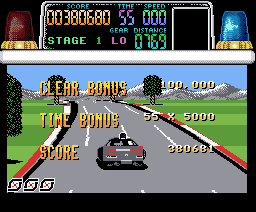
\includegraphics[width=0.48\textwidth]{../img/bonus.png}\hfill
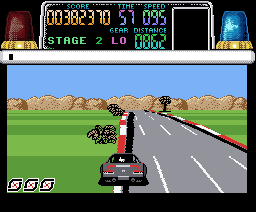
\includegraphics[width=0.48\textwidth]{../img/stage2.png}
\caption{Izquierda: las bonificaciones tras una detención. Derecha: la segunda fase.}
\end{figure}

% ==================================================================
\sect{8. Consejos}

\begin{itemize}
\item Cambia a \texttt{HI} en cuanto te muevas: en \texttt{LO} la velocidad máxima es mucho menor.
\item Guarda los turbos para cuando el criminal esté a la vista: con el turbo puesto conservas más velocidad tras cada golpe.
\item Adelanta sin tocar a los demás coches: un choque te cuesta velocidad, tiempo y los puntos de adelantamiento.
\item No te salgas del asfalto: fuera de la carretera pierdes velocidad, y con ella tiempo.
\item El aviso te dice qué coche lleva el criminal: búscalo entre el tráfico.
\end{itemize}
